\begin{frame}{Модели окружающего пространства}
	В рамках данной работы исследуются \textbf{двухмерные модели} – модели про­ецирующие объекты, окружающие БТС, на плоскость его движения. Как правило, этой информации достаточно для корректного планирования движения БТС.
	
	Среди существующих двумерных моделей можно выделить три категории:
	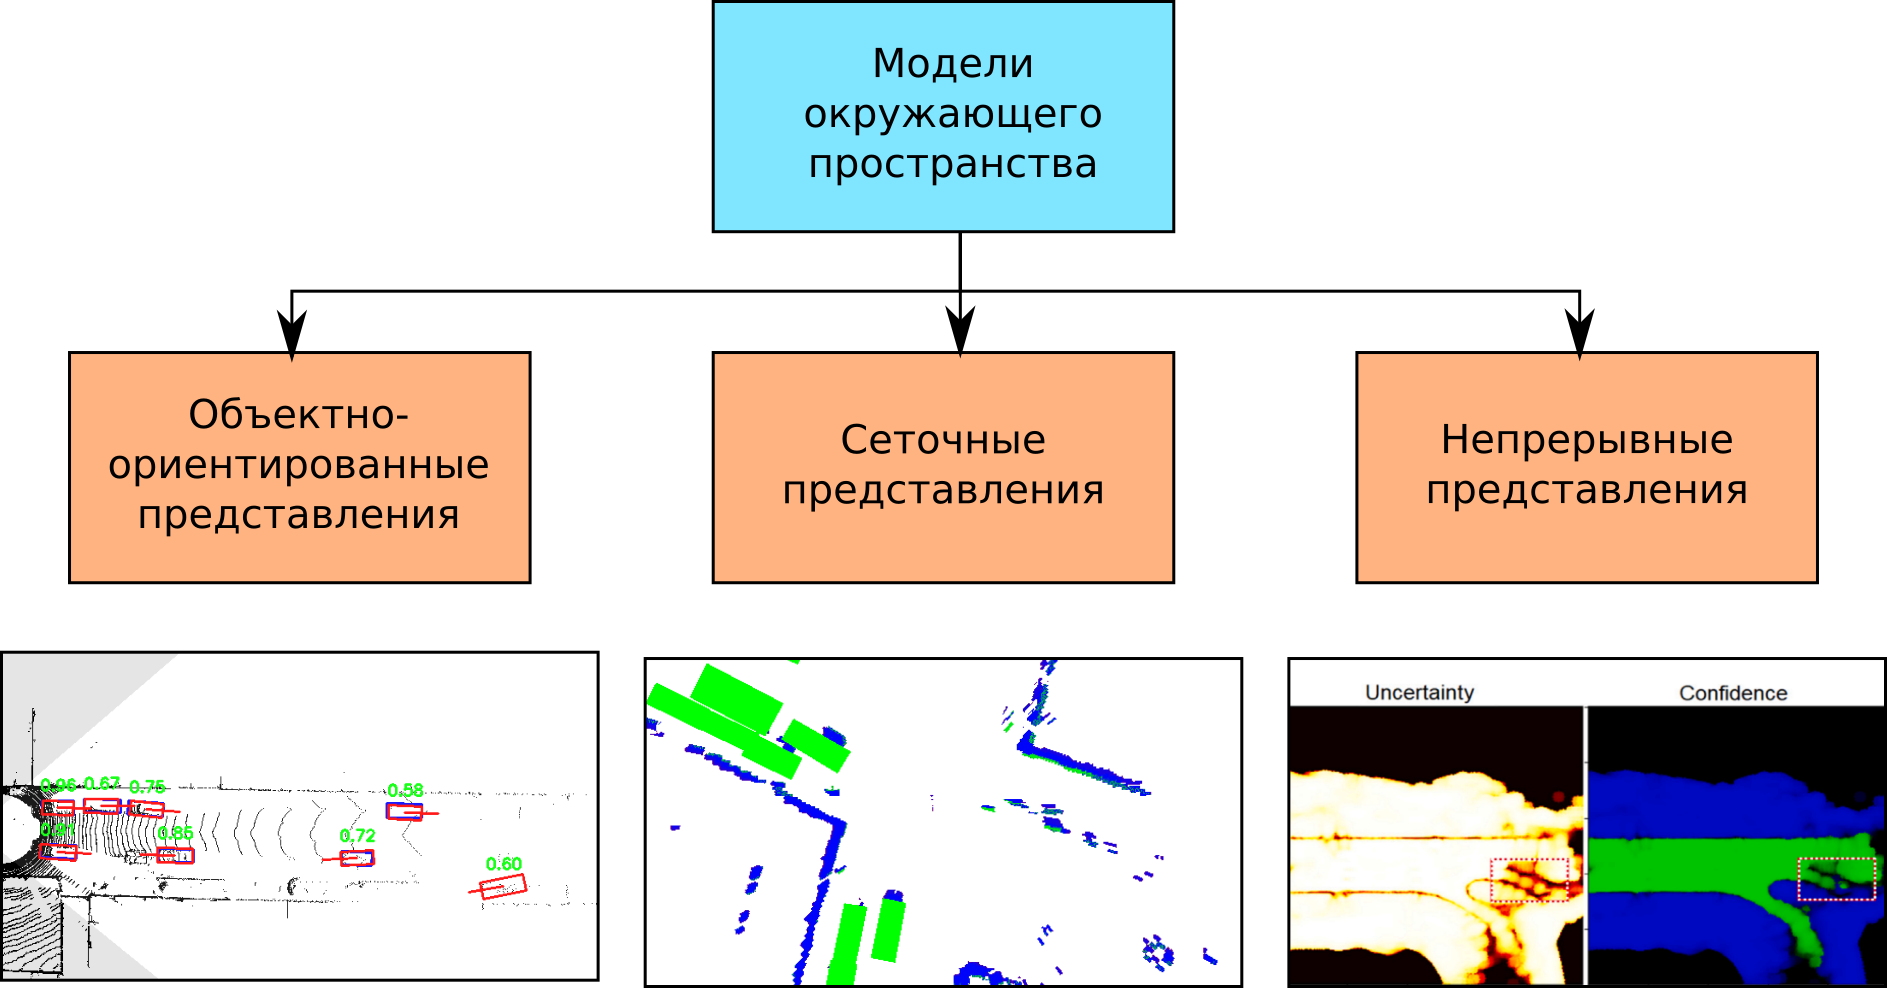
\includegraphics[width=\linewidth]{Presentation/images/models}
\end{frame}

\begin{frame}{Карта проходимости пространства}
	В данном исследования в качестве основной модели взята карта проходимости пространства. В рамках данной модели окружающее БТС пространство разбивается на двумерную сетку $M$, каждой клетке которой $m_i$ сопоставляется вероятность нахождения препятствия в клетке $p(m_i)$. 
	
	\begin{minipage}{0.6\linewidth}	
		Для данной модели делаются следующие  предположения:
		\begin{itemize}
			\item БТС осуществляет движение в плоскости $OXY$;
			\item Каждая клетка карты целиком либо занята, либо свободна;
			\item Значение клетки $m_i$ -- независимая случайная величина;
		\end{itemize}
	\end{minipage}
	\begin{minipage}{0.39\linewidth}
		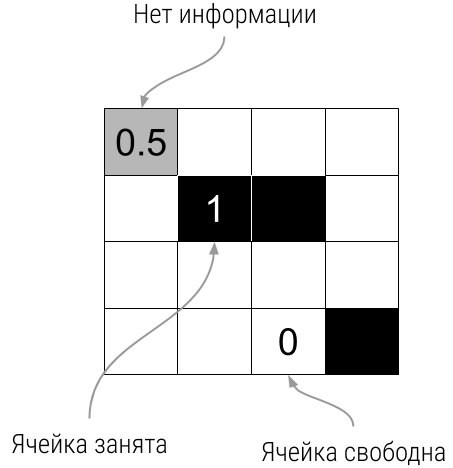
\includegraphics[width=\linewidth]{Presentation/images/map_cells}
	\end{minipage}
	
\end{frame}


\begin{frame}{Задача проекции визуальных детекций на плоскость движения БТС}
	\begin{minipage}{0.6\linewidth}
	\footnotesize
	\textbf{Имея:}
	\begin{itemize}
		\item визуальные детекции окружающих транспортных средств (ТС), полученного с камеры БТС,
		\item семантическую сегментацию проезжей части для этого же изображения,
		\item внутреннюю и внешнюю калибровки камеры,
	\end{itemize}
	\textbf{необходимо оценить} положение окружающих ТС в виде ориентированных ограничивающих рамок на плоскости $OXY$
	
	Для решения задачи делаются следующие предположения:
	\begin{itemize}
		\item все ТС находятся на проезжей части;
		\item поверхность дороги лежит в плоскости $OXY$.
	\end{itemize}
	\end{minipage}
	\begin{minipage}{0.39\linewidth}
		
\includegraphics[width=\linewidth]{projection_task}
	\end{minipage}
\end{frame}

\begin{frame}[allowframebreaks]
	\frametitle{Алгоритм проекции визуальных детекций на плоскость
движения БТС на основе модели L-Shape}
    \small
    \textbf{Впервые предложен} алгоритм оценки положения ТС на плоскость движения БТС на основе модели L-Shape. Алгоритм состоит из двух шагов: 
    \begin{enumerate}
    	\item проекция нижней границы ТС на плоскость движения БТС,
    	\item вписывание полученной проекции в ориентированную ограничивающую рамку.
    \end{enumerate}
    
    Для предлагаемого алгоритма делается дополнительные предположения:
    \begin{enumerate}
    	\item Точки полученной проекции принадлежат двум смежным и ортогональным сторонам ТС,
    	\item Точки проекции упорядочены таким образом, что сперва идут точки принадлежащие одной стороне ТС, затем точки второй стороны.
    \end{enumerate}
    
    \framebreak
    \begin{minipage}{0.5\linewidth}
    	\begin{enumerate}
    		\item Берем $N$ равномерно распределенных точек на нижней границе ограничивающей рамки.
    		\item Каждая полученная точка сдвигается к верху изображения пиксель за пикселем, пока она не выйдет за пределы проезжей.
    		\item Выпуклая оболочка полученных точек проецируется (центральная проекция) на OXY. 
    	\end{enumerate}
    \end{minipage}
    \begin{minipage}{0.49\linewidth}
	\centering
	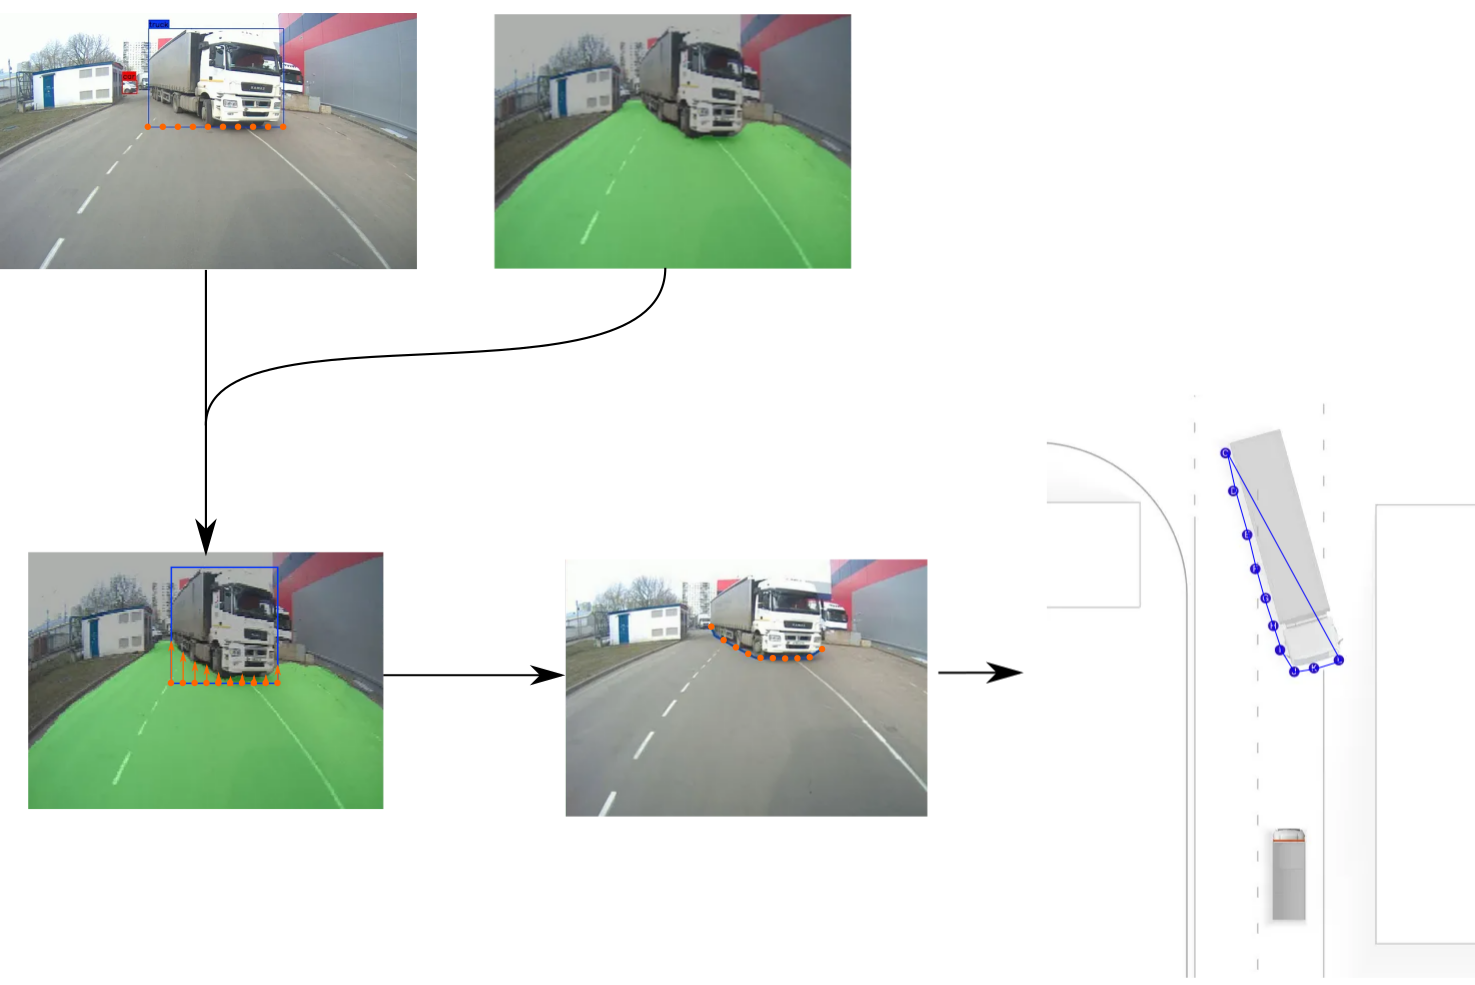
\includegraphics[width=\linewidth]{images/l-shape.png}
	\end{minipage}
	
	\framebreak
	Необходимо оценить параметры двух ортогональных прямых: 
	$l: y = kx + d_1$ и $l': x = -ky+d_2$, таких что минимизируется среднеквадратичное отклонение вписываемых точек до соответствующей прямой.
	
	Согласно сделанным ранее предположениям:
	\begin{align*}
		\exists m \in \{1,\dots,N - 1\}\hookrightarrow& \forall i \in \{1,\dots,m\}, p_i = (x_i, y_i) \in l;\\
		&\forall i \in \{m+1,\dots,N\},p_i = (x_i, y_i) \in l'
	\end{align*}
	
	Для некоторого фиксированного $m$, задача минимизации выглядит следующим образом:
	
	\begin{equation*}
		\operatorname*{argmin}_{k, d_1,d_2}\left(\begin{pmatrix}
			x_1 & 1 & 0 \\
			x_2 & 1 & 0 \\
			\vdots & \vdots  & \vdots  \\
			x_{m} & 1 & 0 \\
			-y_{m + 1} & 0 & 1 \\
			\vdots & \vdots  & \vdots  \\
			-y_{N} & 0 & 1 \\
		\end{pmatrix} 
		\begin{pmatrix}
			k \\
			d_1\\
			d_2 \\
		\end{pmatrix} - \begin{pmatrix}
			y_1 \\
			y_2\\
			\vdots \\
			y_{m} \\
			x_{m + 1} \\
			\vdots \\
			x_{N} \\
		\end{pmatrix}\right)^2    
	\end{equation*}
	
	Введя дополнительные обозначения, мы можем переписать это выражение следующим образом:
	
	\begin{equation*}
		\operatorname*{argmin}_{a}\left(\begin{pmatrix}
			\widehat{x} & 1 & 0 \\
			-\widehat{y} & 0 & 1 \\
		\end{pmatrix} 
		a - \begin{pmatrix}
			\widetilde{y} \\
			\widetilde{x} \\
		\end{pmatrix}\right)^2
	\end{equation*}
	
	И далее:
	
	\begin{equation*}
		\operatorname*{argmin}_{a}\left(Xa - y \right)^2
	\end{equation*}
	
	Решением данной задачи минимизации является:
	
	\begin{align}
		a^* &= \left(X^TX\right)^{-1}X^Ty \label{eq:optimal_lsh_sol}\\
		\text{MSE} &= a^{*T}X^TXa - 2 a^{*T}X^Ty - y^Ty \label{eq:optimal_lsh_sol_mse}
	\end{align}
	
	\framebreak
	Итоговый алгоритм вписывания проекции в рамку имеет следующий вид:
	
	\begin{enumerate}
		\item Перебираем все значения $m \in \{1,\dots,N-1\}$
		\item Пересчитываем матрицы $X,y$
		\item Находим $a^*$, MSE для каждой задачи минимизации по формулам~\ref{eq:optimal_lsh_sol},\ref{eq:optimal_lsh_sol_mse}
		\item В качестве финального решения для $l, l'$ выбираем $a^*$ с наименьшим MSE.
		\item Обрамляем вписываемый набор точек линиями параллельными $l$ и $l'$. Область ограниченная полученными линиями -- искомая ограничивающая рамка.
	\end{enumerate}
	
	\textbf{В работе предложена реализация }алгоритма, имеющая вычислительную сложность $O(N)$, где $N$ -- число точек вписываемой проекции.
\end{frame}

\begin{frame}{Экспериментальное исследование для БТС. Данные}
	\begin{itemize}
		\item Объектом испытаний было грузовое БТС «EVO.1»;
		\item Подготовлен тестовый набор с реальными сценами из $4$ локаций, $12$ видеопоследовательностей, $93$ кадров. 
		\item Набор включает вручную размеченные эталонные значения положения окружающих ТС.
	\end{itemize}
	\centering
	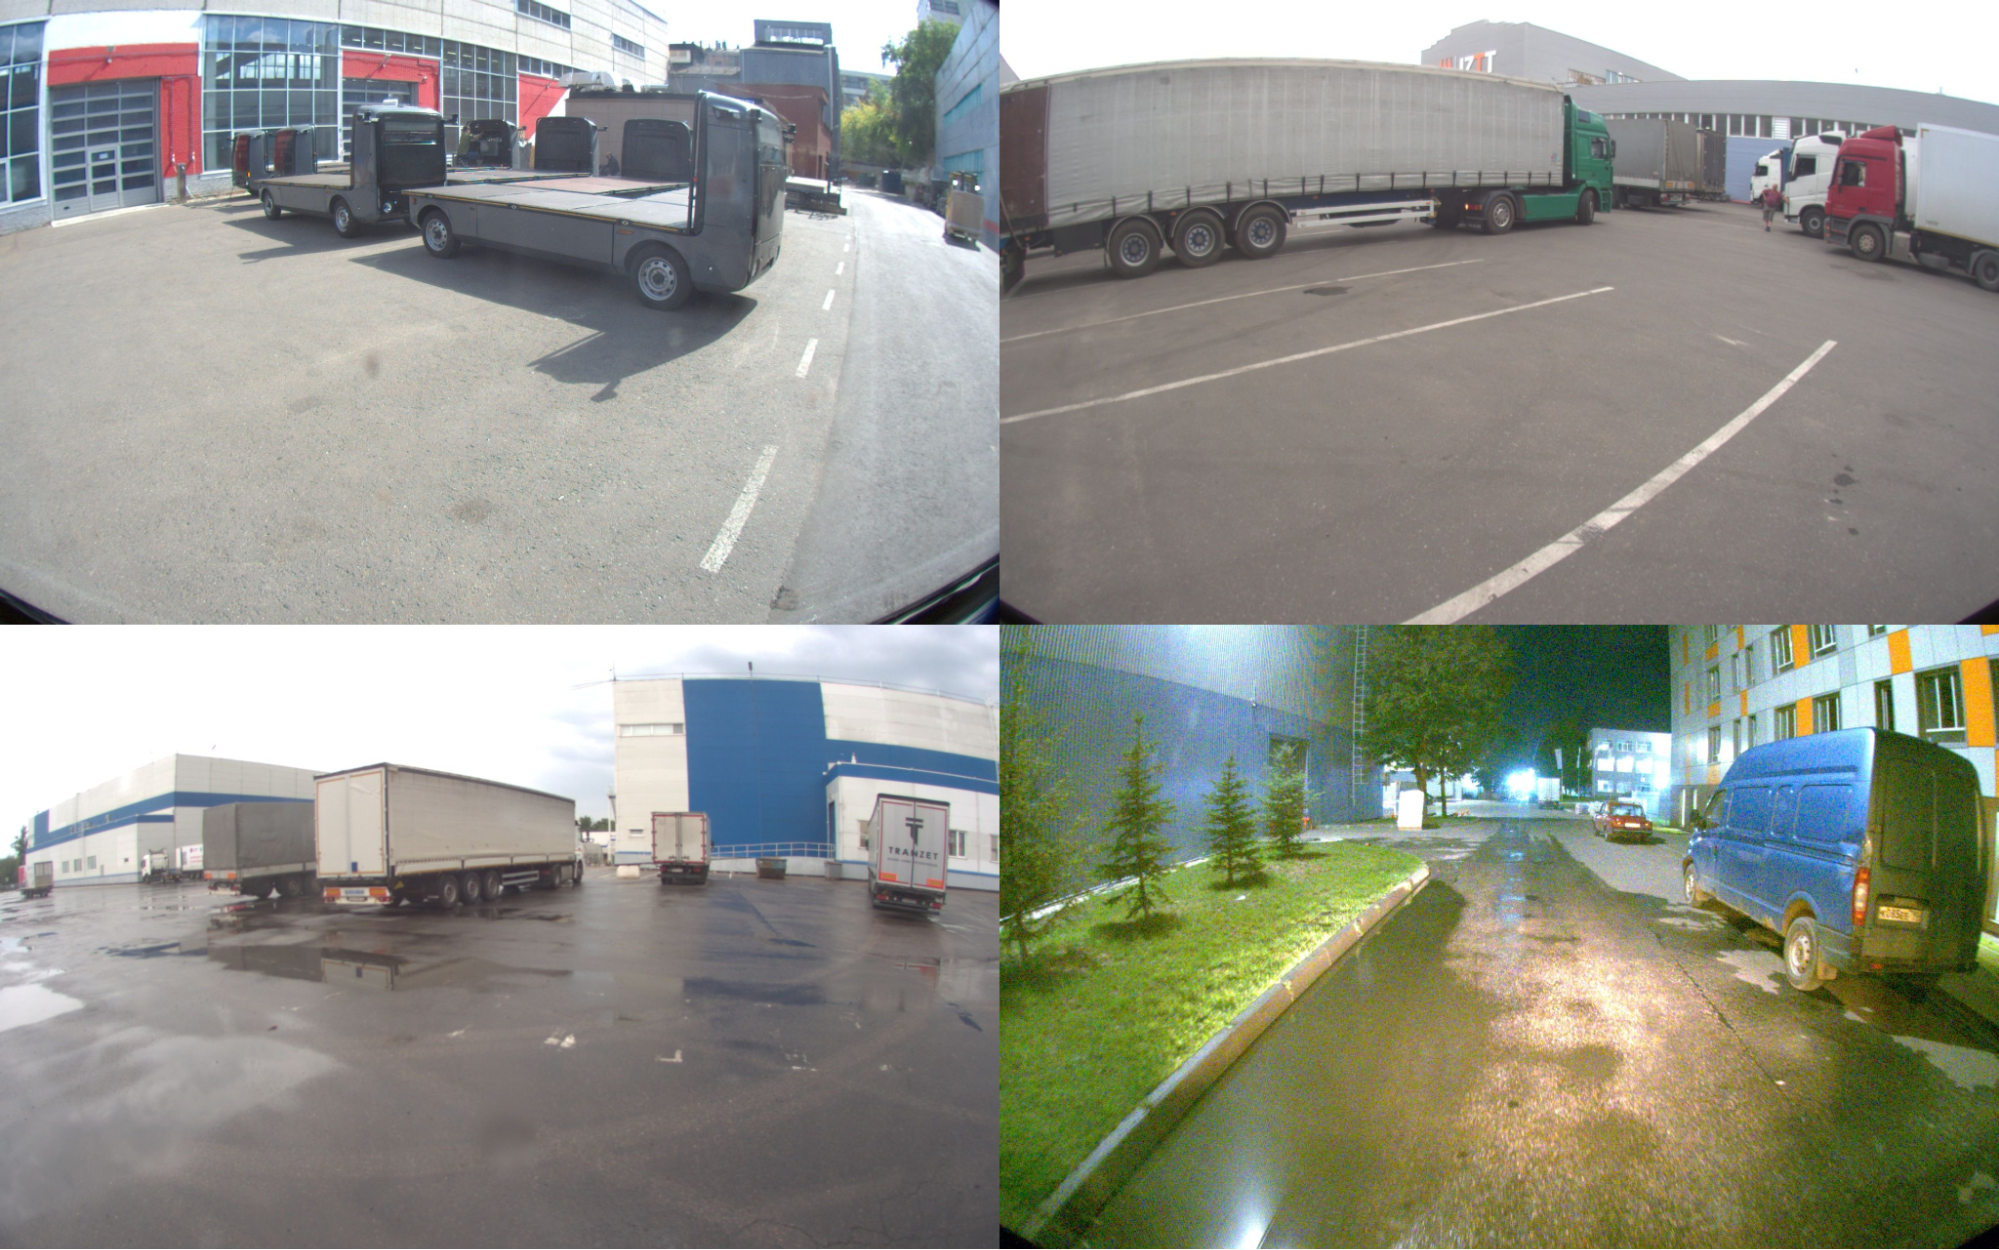
\includegraphics[width=0.8\linewidth]{images/scenes.png}
\end{frame}


\begin{frame}{Экспериментальное исследование для БТС. Методология}
	\begin{itemize}
		\item Исследовалось качество второго этапа алгоритма: вписывание проекции в ограничивающую рамку.
		\item Предложенный алгоритм сравнивался с пятью подходами:
		\begin{itemize}
			\item наивный подход поиска рамки минимальной площади,
			\item четыре алгоритма оценки положения ТС из работы, посвящённой схожей задаче для лидарных облаков точек\footnote{Optimal Vehicle Pose Estimation Network Based on Time Series and Spatial Tightness with 3D LiDARs [Текст] / H. Wang [и др.] // Remote Sensing. — 2021.}.
		\end{itemize}
		\item Для оценки качества алгоритма использовался усреднённое значение коэффициента Жаккара:
		$$IoU(prDet,gtDet) = \dfrac{S(prDet\cap gtDet)}{S(prDet\cup gtDet)},$$
		где $prDet$ -- построенная рамка, $gtDet$ -- эталонная рамка, $S(x)$ -- площадь многоугольника $x$.
	    \item Дополнительно исследовалось качество всех сравниваемых алгоритмов при ограничении расстояния до ТС.
	\end{itemize}
\end{frame}

\begin{frame}[allowframebreaks]
	\frametitle{Экспериментальное исследование для БТС. Результаты}
		\begin{table}[h!]
			\small
			\centering
			\begin{tabular}{|p{0.1\textwidth}|p{0.11\textwidth}|p{0.1\textwidth}|p{0.11\textwidth}|p{0.11\textwidth}|p{0.12\textwidth}|p{0.11\textwidth}|}
				\hline
				           & \textbf{Мин. площадь} & \textbf{Rotating PCA} & \textbf{Diagonal PCA} & \textbf{Longest Diagonal} & \textbf{Rotated Triangle} & \textbf{L-Shape}\\
				\hline
				Среднее & $0.294\newline(-12.8\%)$ & $0.328\newline(-2.7\%)$ & $0.321\newline(-4.7\%)$ & $0.323\newline(-4.2\%)$ & $0.301\newline(-10.7\%)$ & \boldmath$0.337\newline(-0.0\%)$ \\
				\hline
		    	 $\sigma$ & $0.146$ & $0.144$ & $0.149$ & $0.156$ & $0.141$ & $0.141$ \\
				\hline
				Мин. & $0.059\newline(-24.4\%)$  & $0.075\newline(-3.8\%)$ & \boldmath$0.078\newline(-0.0\%)$ & $0.074\newline(-5.1\%)$ & $0.059\newline(-24.4\%)$ & \boldmath$0.078\newline(-0.0\%)$\\
				\hline
				$25\%$ & $0.198\newline(-13.9\%)$ & $0.219\newline(-4.8\%)$ & $0.202\newline(-12.2\%)$ &$0.199\newline(-13.5\%)$ & $0.208\newline(-9.6\%)$ & \boldmath$0.230\newline(-0.0\%)$ \\
				\hline
				$50\%$ & $0.257\newline(-21.6\%)$ & $0.316\newline(-3.7\%)$ & $0.316\newline(-3.7\%)$ & $0.287\newline(-12.5\%)$ & $0.264\newline(-19.5\%)$ & \boldmath$0.328\newline(-0.0\%)$ \\
				\hline
				$75\%$ & $0.383\newline(-15.1\%)$ & $0.448\newline(-0.7\%)$ & $0.445\newline(-1.3\%)$ & $0.442\newline(-2.0\%)$ & $0.425\newline(-5.8\%)$ & \boldmath$0.451\newline(-0.0\%)$ \\	
				\hline
				Макc. & $0.649\newline(-9.0\%)$ & $0.607\newline(-14.9\%)$ & $0.622\newline(-12.8\%)$ & $0.651\newline(-8.7\%)$ & $0.579\newline(-18.8\%)$ & \boldmath$0.713\newline(-0.0\%)$ \\
				\hline
			\end{tabular}
		\end{table}
		
	\framebreak
	\begin{minipage}{0.4\linewidth}
		\begin{itemize}
			\item На тестовом наборе данных \textbf{показано}, что предлагаемый алгоритм превосходит аналоги: ближайший алгоритм имеет усреднённый коэффициент Жаккара на $2.7\%$ ниже.
			\item \textbf{Показано}, что качество всех алгоритмов начинает снижаться после при оценке положения ТС, расположенных далее $10$ метров.
		\end{itemize}
	\end{minipage}	
	\begin{minipage}{0.59\linewidth}
		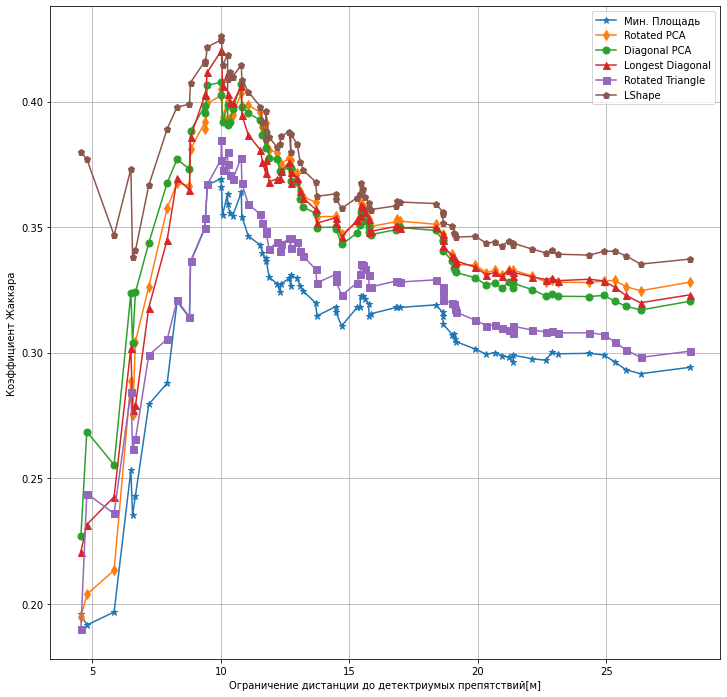
\includegraphics[width=\linewidth]{images/l-shape_metrics}
	\end{minipage}
\end{frame}

\begin{frame}{Задача проекции визуальных детекций на плоскость движения БТС на основе комплексирования данных камеры и лидаров}
\begin{minipage}{0.5\linewidth}
	\textbf{Имея:}
	\begin{itemize}
		\item визуальные детекции окружающих транспортных средств (ТС), полученного с камеры БТС,
		\item внутреннюю и внешнюю калибровки камеры,
		\item \textbf{облако точек, полученного с лидаров БТС}
	\end{itemize}
	\textbf{необходимо оценить} положение окружающих ТС в виде ориентированных ограничивающих рамок на плоскости $OXY$
	
	
\end{minipage}
\begin{minipage}{0.49\linewidth}
	
\includegraphics[width=\linewidth]{projection_with_lidars_task}
\end{minipage}		
\end{frame}

\begin{frame}{Алгоритм проекции визуальных детекций на плоскость движения БТС на основе комплексирования данных камеры и лидаров}
	\footnotesize
	\IncMargin{2em}
	\begin{minipage}{\linewidth}
	\begin{algorithm}[H]
		\LinesNumbered
		\KwIn{$\{d_1,\dots d_n\}$ -- визуальные детекции, $P$ -- облако точек.}
		\KwOut{$b_i$ -- ориентированные ограничивающие рамки на виде сверху окружающих БТС объектов.}
		Выделить в облаке точек $P$ точки, не принадлежащие поверхности земли: $P_o$\;
		Кластеризовать полученное облако точек $P_o$;
		Спроецировать все кластеры на изображение $I$: $C_i \rightarrow \widehat{C}_i$.;
		Для каждого спроецированного кластера найти ограничивающую рамку минимального размера: $d_{C_i}$\;
		Используя Венгерский алгоритм найти наилучшее сопоставление $d_i$ с  $d_{C_i}$;
		В оставшихся кластерах удалить точки, не попадающие при проекции в сопоставленную детекцию $d_i$: $C_i \rightarrow C^-_i$.\;
		\ForEach{$C^-_i$}{
			Используя RANSAC(RANdom SAmple Consensus) найти прямую $l_i$ в $C^-_i$.\;
			Построить ограничивающую рамку $b_i$, со сторонами параллельными $l_i$ и ортогональной ей $l'_i$.\;
		}
		\Return{$\{b_i\}$}
	\end{algorithm}
	\end{minipage}
\end{frame}

\begin{frame}{Пример результата работы алгоритма}
	\centering
	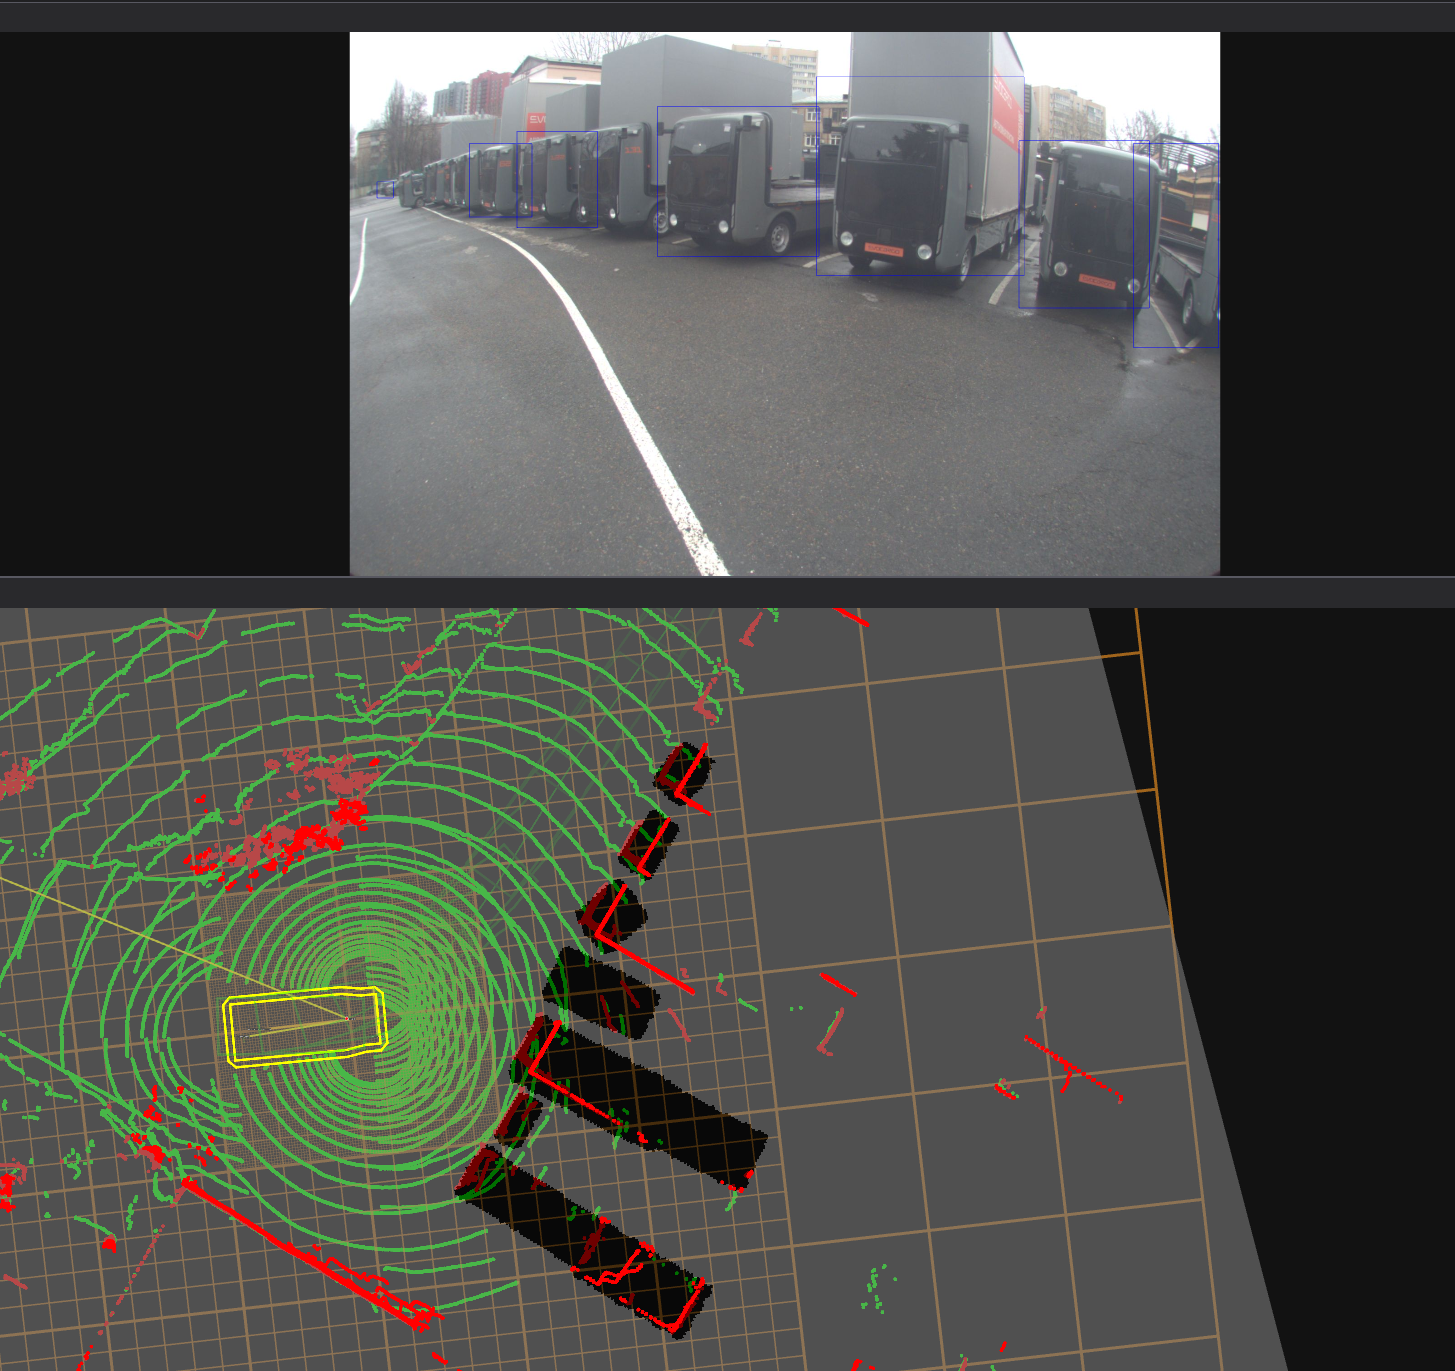
\includegraphics[width=0.8\linewidth]{images/true3ddet_demo}
\end{frame}

\begin{frame}{Задача проекции сегментации проезжей части на
		изображении на плоскость движения TC}
	\begin{minipage}{0.5\linewidth}
		\textbf{Имея:}
		\begin{itemize}
			\item семантическую сегментацию проезжей части на изображении с камеры БТС,
			\item внутреннюю и внешнюю калибровки камеры,
			\item \textbf{облако точек, полученного с лидаров БТС}
		\end{itemize}
		\textbf{необходимо оценить} проекцию проезжей части на плоскость движения БТС
	\end{minipage}
	\begin{minipage}{0.49\linewidth}
		
\includegraphics[width=\linewidth]{projection_segmentation_task}
	\end{minipage}
\end{frame}

\begin{comment}
\section{Списки}
\begin{frame}[plain, noframenumbering]
    \begin{center}
        \Huge
        Списки
    \end{center}
\end{frame}

\subsection{Нумерованные}

\begin{frame}
    \frametitle{Нумерованные списки}
    \begin{enumerate}
        \item один
        \item два
        \item три
    \end{enumerate}
\end{frame}
\note{
    Этот текст будет виден только если его отображение включено
    в~файле \textbf{Presentation/setup}.
    Для раздельного вывода презентации и заметок на~разные экраны (как
    в~impress или powerpoint) можно использовать программу
    \textit{pdf-presenter-console}.
}

\subsection{Не нумерованные}


\begin{frame}
    \frametitle{Перечисления}
    \begin{itemize}
        \item Проблема 1
        \item Проблема 2
        \item Проблема 3
    \end{itemize}
\end{frame}
\note[itemize]{
    \item Тезис 1
    \item Тезис 2
    \item Тезис 3
}

\subsection{Комбинированные}

\begin{frame}
    \frametitle{Комбинация списков}
    \begin{enumerate}
        \item \textbf{Задача 1}
              \begin{itemize}
                  \item Подзадача 1-1
                  \item Подзадача 1-2
              \end{itemize}
        \item \textbf{Задача 2}
              \begin{itemize}
                  \item Подзадача 2-1
                  \item Подзадача 2-2
                  \item Подзадача 2-3
              \end{itemize}
        \item \textbf{Задача 3}
              \begin{itemize}
                  \item Подзадача 3-1
                  \item Подзадача 3-2
                  \item Подзадача 3-3
              \end{itemize}
    \end{enumerate}
\end{frame}
\note[itemize]{
    \item Задача 1
    \item Задача 2
    \item Задача 3
}

\begin{frame}[allowframebreaks]
    \frametitle{Разделение слайда}
    Поясняющий текст
    \begin{itemize}
        \item Один
        \item Два
        \item Три
    \end{itemize}
    \framebreak
    Продолжение предыдущего слайда
\end{frame}

\section{Графика}
\begin{frame}[plain, noframenumbering]
    \begin{center}
        \Huge
        Графика
    \end{center}
\end{frame}


\begin{frame}
    \frametitle{Одиночное изображение}
    \centering
    \includegraphics[width=0.8\linewidth]{latex} % окружение figure не требуется
\end{frame}

\begin{frame}
    \frametitle{Векторная графика}
    \begin{figure}
        \centering
        \ifdefmacro{\tikzsetnextfilename}{\tikzsetnextfilename{tikz_presentation}}{}% присваиваемое предкомпилированному pdf имя файла (не обязательно)
        \input{Presentation/images/tikz_plot.tikz}
    \end{figure}
\end{frame}

\subsection{Расположение}

\begin{frame}
    \frametitle{Изображения по-вертикали}
    \centering
    \vfill
    \includegraphics[width=0.8\linewidth,height=0.1\textheight]{latex} \\
    \TeX
    \vfill
    \includegraphics[width=0.8\linewidth,height=0.2\textheight]{latex} \\
    \LaTeX
    \vfill
    \includegraphics[scale=0.2]{latex} \\
    \vfill
\end{frame}


\begin{frame}
    \frametitle{Изображения по-горизонтали}
    \begin{minipage}[t]{0.47\linewidth}
        \textbf{Составная \\ подпись 1}
        \center{\includegraphics[width=1\linewidth]{knuth1}}
    \end{minipage}
    \hfill
    \begin{minipage}[t]{0.47\linewidth}
        \textbf{Составная \\ подпись 2}
        \center{\includegraphics[width=1\linewidth]{knuth2}}
    \end{minipage}
\end{frame}

\subsection{Линии}

\begin{frame}
    \frametitle{Разделяющие линии}
    \begin{minipage}[c]{0.47\linewidth}
        \center{\includegraphics[width=1\linewidth]{latex}}
        \bigskip
        \hrule{}
        \bigskip
        \textbf{Составная \\ подпись 1}
    \end{minipage}
    \hfill
    \vrule{}
    \hfill
    \begin{minipage}[c]{0.47\linewidth}
        \flushright
        \textbf{Составная \\ подпись 2}
        \center{\includegraphics[width=1\linewidth]{knuth2}}
    \end{minipage}
\end{frame}

\section{Остальное}
\begin{frame}[plain, noframenumbering]
    \begin{center}
        \Huge
        Остальное
    \end{center}
\end{frame}

\subsection{Формулы}

\begin{frame}
    \frametitle{Формулы}
    \[
    \left\{
    \begin{array}{rl}
        \dot x = & \sigma (y-x)  \\
        \dot y = & x (r - z) - y \\
        \dot z = & xy - bz
    \end{array}
    \right.
    \]
\end{frame}

\begin{frame}
    \frametitle{amsmath}
    \centering
    \begin{minipage}[t]{0.5\linewidth}
        \begin{multline*}
            y = 1 x^1 + 2 x^2 + 3 x^3 + \\ + 4 x^4 + 5 x^5 + \dots
        \end{multline*}
    \end{minipage}
\end{frame}

\begin{frame}[allowframebreaks]
    \frametitle{Уравнения Максвелла}
    \centering{
        \small
        \def\arraystretch{1.8}%
        \begin{tabular}{ll}
            \toprule
            Интегральная форма                                                                                                                                            & Дифференциальная форма                                                          \\ \midrule
            \(Q_e(t) = \displaystyle\oiint_S \vec D(t) \cdot d\vec{s} = \displaystyle\iiint_V \rho_v(t) dv\)                                                              & \(\nabla \cdot \vec D(t) = \rho_v(t)\)                                          \\
            \(\displaystyle\oiint_S \vec B(t) \cdot d\vec{s} = 0\)                                                                                                        & \(\nabla \cdot \vec B(t) = 0\)                                                  \\
            \(V_{emf}(t) = \displaystyle\oint_L \vec E(t) \cdot d\vec{l}\) = \(- \displaystyle\iint_S \left[\frac{\partial\vec{B}(t)}{\partial t}\right] \cdot d\vec{s}\) & \(\nabla \times \vec E(t) = - \frac{\partial\vec{B}(t)}{\partial t}\)           \\
            \(I(t) = \displaystyle\oint_L \vec H(t) \cdot d\vec{l} = \displaystyle\iint_S \left[\vec J(t) + \frac{\partial\vec{D}(t)}{\partial t}\right] \cdot d\vec{s}\) & \(\nabla \times \vec H(t) = \vec J(t) + \frac{\partial\vec{D}(t)}{\partial t}\) \\ \midrule
            \(\displaystyle\oiint_S \vec J \cdot d\vec{s} = -\frac{\partial Q_e}{\partial t}\)                                                                            & \(\nabla \cdot \vec J = - \frac{\partial \rho_v}{\partial t}\)                  \\
            \bottomrule
            \multicolumn{2}{c}{\(\vec D(t) = \left[\varepsilon(t)\right] * \vec E(t)\)}                                                                                                                                                                     \\
            \multicolumn{2}{c}{\(\vec B(t) = \left[\mu(t)\right] * \vec H(t)\)}                                                                                                                                                                             \\
        \end{tabular}
    }
    \framebreak

    \hspace{0.05\linewidth}
    \centering{
        \small
        \def\arraystretch{1.8}%
        \begin{tabular}{ll}
            \toprule
            Интегральная форма                                                                                                                & Дифференциальная форма                               \\ \midrule
            \(Q_e = \displaystyle\oiint_S \vec D \cdot d\vec{s} = \displaystyle\iiint_V \rho_v dv\)                                           & \(\nabla \cdot \vec D = \rho_v\)                     \\
            \(\displaystyle\oiint_S \vec B \cdot d\vec{s} = 0\)                                                                               & \(\nabla \cdot \vec B = 0\)                          \\
            \(V_{emf} = \displaystyle\oint_L \vec E \cdot d\vec{l}\) = \(- \displaystyle\iint_S \left[j \omega \vec B\right] \cdot d\vec{s}\) & \(\nabla \times \vec E = - j \omega \vec B\)         \\
            \(I = \displaystyle\oint_L \vec H \cdot d\vec{l} = \displaystyle\iint_S \left[\vec J + j \omega \vec D\right] \cdot d\vec{s}\)    & \(\nabla \times \vec H = \vec J + j \omega \vec{D}\) \\ \midrule
            \(\displaystyle\oiint_S \vec J \cdot d\vec{s} = - j \omega Q_e\)                                                                  & \(\nabla \cdot \vec J = - j \omega \rho_v\)          \\
            \bottomrule
            \multicolumn{2}{c}{\(\vec D(t) = \left[\varepsilon\right] \vec E(t)\)}                                                                                                                   \\
            \multicolumn{2}{c}{\(\vec B(t) = \left[\mu\right] \vec H(t)\)}                                                                                                                           \\
        \end{tabular}
    }
\end{frame}

\subsection{Таблицы}

\begin{frame}
    \frametitle{Таблица}
    \centering
    \begin{tabular}{|l|l|}
        \hline
        \textbf{Заголовок 1} & \textbf{Заголовок 2} \\
        \hline
        Сумма                & \(b+a\)              \\
        \hline
        Разность             & \(a-b\)              \\
        \hline
        Произведение         & \(a*b\)              \\
        \hline
    \end{tabular}
\end{frame}

\begin{frame}
    \frametitle{Другая таблица}
    \centering
    \begin{tabular}{lc}
        \toprule
        \multicolumn{1}{c}{\textbf{Заголовок 1}} & \textbf{Заголовок 2} \\ \midrule
        Сумма                                    & \(b+a\)              \\
        Разность                                 & \(a-b\)              \\
        Произведение                             & \(a*b\)              \\
        \bottomrule
    \end{tabular}
\end{frame}


\subsection{Разное}

\begin{frame}
    \frametitle{Большой многоуровневый список}
    \begin{itemize}
        \item \textbf{Пункт 1}
              \begin{itemize}
                  \itemi Подпункт 1-1
                  \itemi Подпункт 1-2
              \end{itemize}
        \item \textbf{Пункт 2}
              \begin{itemize}
                  \itemi Подпункт 2-1
              \end{itemize}
        \item \textbf{Пункт 3}
              \begin{itemize}
                  \itemi Подпункт 3-1
                  \itemi Подпункт 3-2
              \end{itemize}
        \item \textbf{Пункт 4}
              \begin{itemize}
                  \itemi Подпункт 4-1
              \end{itemize}
        \item \textbf{Пункт 5}
              \begin{itemize}
                  \itemi Подпункт 5-1
                  \itemi Подпункт 5-2
                  \itemi Подпункт 5-3
              \end{itemize}
    \end{itemize}
\end{frame}

\begin{frame}
    \frametitle{Четыре изображения}
    \centering
    \includegraphics[width=0.35\linewidth,angle=35]{latex}
    \includegraphics[width=0.35\linewidth,angle=135]{latex}\\
    \includegraphics[width=0.35\linewidth,angle=15]{latex}
    \includegraphics[width=0.35\linewidth,angle=-15]{latex}
\end{frame}

\end{comment}